\chapter{Schiefe Ebene}

Die schiefe Ebene stellt ein klassisches Problem der Mechanik. 
Diese kombiniert einfache Kräftebetrachtungen und zeigt den 
vektoriellen Charakter von Kräften und Beschleunigungen auf, welche sich 
mit der Anwendung trigonometrischer Gesetze bestimmen lassen.

\newpage
\section{Kräfte am Hang}
\begin{figure}[h!]
	\centering
	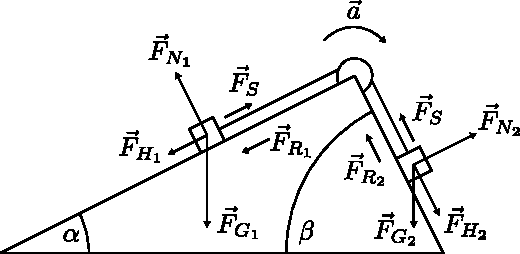
\includegraphics[scale=1]{schiefe-ebene-1.pdf}
	\caption{Kräftesystem mit zwei Massen am Hang}
	\label{fig:hangsystem}
\end{figure}

\subsection{Gewichtskraft}
Die Gewichtskraft gilt am Hang genau gleich wie auf der waagerechten Ebene.
\[ \boxed{\vec{F}_G = m \cdot \vec{g}} 
	\qquad \vec{g} = \vec{a}_{Erde} \approx 9.81\frac{m}{s^2} \]

\subsection{Normalkraft}
Die Normalkraft ist jene Kraftkomponente, welche von der Unterlage senkrecht
durch den Schwerpunkt der Masse geht, welche sie trägt. Somit ist die 
Normalkraft eine Funktion des Neigungswinkels und der Gewichtskraft, d.h.
$\vec{F}_N = f(\vec{F}_G, \alpha)$.
\[ \boxed{ \vec{F}_N 
	= \vec{F}_G \cdot cos(\alpha) 
	= m \cdot \vec{g} \cdot cos(\alpha)} 
\]
\[ \begin{array}{ll}
	\alpha \rightarrow 0 & \Rightarrow \vec{F}_N = \vec{F}_G \\
	\alpha \rightarrow \pi & \Rightarrow \vec{F}_N = 0
\end{array} \]

\subsection{Hangkraft}
Die Hangkraft ist jene Kraftkomponente, welche parallel zur Unterlage in 
Richtung der Gravitation zeigt. Die Wirkungslinie geht dabei wie bei der 
Normalkraft duch den Schwerpunkt der Masse und ist ebenfalls eine Funktion
des Neigungswinkels und der Gewichtskraft, d.h. 
$\vec{F}_N = f(\vec{F}_G, \alpha)$.
\[ \boxed{ \vec{F}_H  
	= \vec{F}_G \cdot sin(\alpha) 
	= m \cdot \vec{g} \cdot sin(\alpha)} 
\]
\[ \begin{array}{ll}
	\alpha \rightarrow 0 & \Rightarrow \vec{F}_N = 0 \\
	\alpha \rightarrow \pi & \Rightarrow \vec{F}_N = \vec{F}_G
\end{array} \]

\subsection{Seilkraft}
Die Seilkraft welche zwischen zwei miteinander verbundenen Massen auftritt
ist überall im Seil die selbe und zieht mit gleichem Betrag an beiden Massen.
\[ \vec{F}_S = |\vec{F}_{S_1}| = |\vec{F}_{S_2}| \]
Die Summe der Seilkräfte (es gibt maximal zwei) muss also folglich Null ergeben.
\[ \sum_{i=1}^{n=2} \vec{F}_{S_i} = \vec{F}_{S_1} + \vec{F}_{S_2} = 0 \]

\subsection{Reibungskraft}
Die Reibungskraft wirkt stets entgegen der Bewegungsrichtung (bremsend) und ist
definiert als das Produkt aus der Normalkraft $\vec{F}_N$ und dem 
Reibungskoeffizienten $\mu$. Beim Reibungskoeffizienten wird  zwischen 
Haft- und Gleitreibung unterschieden ($\mu_{HR}$ und $\mu_{GR}$).
\[ \boxed{\vec{F}_R = \vec{F}_N \cdot \mu} \]

\subsection{Lösungsvorgehen}
Um ein Hangproblem wie im Bild \ref{fig:hangsystem} zu lösen kann die folgende
Methode angewendet werden.
\begin{enumerate}
	\item Qualitative Skizze erstellen mit sämtlichen Kräften.
	\item Jede Masse inkl. zugehörigen Kräften als eigenes System kennzeichnen.
	\item Systembezogene Gleichungen aufstellen in der Form
		\[ \begin{array}{ll}
			m_1 \cdot \vec{a} & = -\vec{F}_{H_1} -\vec{F}_{R_1} +\vec{F}_S \\
			m_2 \cdot \vec{a} & = +\vec{F}_{H_2} -\vec{F}_{R_2} -\vec{F}_S \\
		\end{array} \]
		wobei nur jene Kräfte summiert werden welche in der Wirkungslinie liegen.
	\item Gleichungssystem lösen durch Addition.
		\[ \vec{a}(m_1 + m_2) = 
			-\vec{F}_{H_1} +\vec{F}_{H_1} -\vec{F}_{R_1} +\vec{F}_{R_2} \]
		\[  \vec{a} = \frac{\sum \vec{F}}{\sum m} \]
	\item Seilkräfte bestimmen mittels der ermittelten Beschleunigung $\vec{a}$.
		\[ \vec{F}_S = \dots \]
\end{enumerate}
